\section{Introduction}

\begin{figure*}[t]
\centering
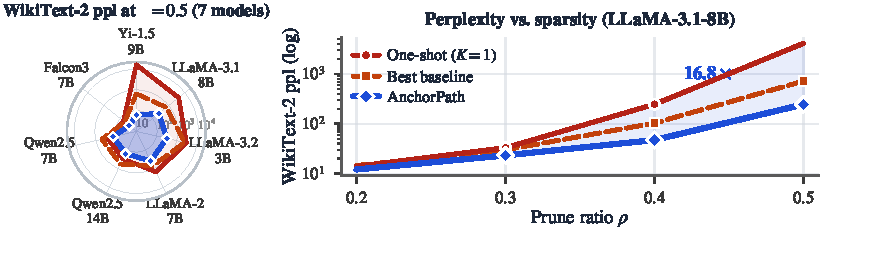
\includegraphics[width=\textwidth]{figs/fig_headline.pdf}
\caption{\textbf{Headline} (calibration-only, no recovery). \textbf{Left:} at $50\%$ pruning across all seven models (radius $=\log$ WikiText-2 ppl), \method (blue) stays a small core inside both one-shot selection (red) and the strongest external baseline (amber). \textbf{Right:} the three methods versus prune ratio on LLaMA-3.1-8B, where the gap widens to $\mathbf{16.8\times}$ below one-shot at $\rho{=}0.5$ with zero weight updates.}
\label{fig:headline}
\end{figure*}

Large language models (LLMs) are expensive to deploy at their pretrained scale, motivating a large body of
work on compressing a \emph{pretrained} model without retraining
it~\citep{vaswani2017attention,frantar2023sparsegpt,sun2024wanda}. \emph{Structured} pruning, which removes
whole computational units such as attention heads and feed-forward (FFN) channel groups, is the form that
yields real wall-clock and memory savings on commodity hardware, unlike unstructured sparsity that needs
special kernels~\citep{ma2023llmpruner,an2024flap,ashkboos2024slicegpt}. Yet it has a stubborn ceiling:
accuracy collapses once a moderate fraction of units is removed. We identify the cause and show the
collapse can be defeated by a better \emph{selection} of what to remove, with no weight updates.

\paragraph{The ceiling.}
Calibration-only structured pruners are reliable only at \emph{low} sparsity:
Taylor-saliency~\citep{ma2023llmpruner,molchanov2019taylor},
activation-fluctuation~\citep{an2024flap,sun2024wanda}, and rotation~\citep{ashkboos2024slicegpt} methods
all collapse at moderate sparsity, which is exactly why the strongest of them
append LoRA or post-pruning fine-tuning. That recovery stage is a tacit admission: the importance ranking
computed on the dense model ceases to be trustworthy as pruning proceeds. Our question is therefore not
``which score is best?'' but \emph{why does structured pruning collapse at high sparsity at all?}

\paragraph{Insight 1: the collapse is a property of the \emph{paradigm}, not the score.}
The methods above, and the standard no-recovery pruners generally, share one move: each builds a
\emph{single} local model of the pruning loss at the dense operating point (a first- or second-order
Taylor expansion, or an equivalent activation statistic), then ranks \emph{all} units against that one
model and deletes a whole budget's worth of them in one shot. A local quadratic is faithful only near its
expansion point; deleting $40$ to $50\%$ of the units carries the model far outside that neighborhood, so a
saliency accurate at the dense model loses validity. The failure has a distinctive signature: measured
against the dense model, post-pruning perplexity grows not linearly but \emph{super-exponentially} in the
prune ratio. On LLaMA-2-7B the per-$10\%$ inflation factor itself accelerates, with perplexity reaching
$1497$ at $\rho{=}0.5$ (Sec.~\ref{sec:superexp}). A collapse whose \emph{rate} accelerates cannot be patched by a
better one-shot score; it is the geometry of extrapolation, shared by the entire family.

% \paragraph{Insight 2: follow the budget, do not extrapolate across it.}
% If a single quadratic cannot span the budget, we abandon it. We recast structured compression from a
% one-shot \emph{selection} problem into a calibration-only \emph{continuation}: follow a cost-indexed
% sequence of pruning states, refreshing current-model ablation perturbations at each partially pruned model
% (a classical path-tracing idea~\citep{mo2023spode} instantiated here with a fixed dense-anchor Fisher
% metric). The conceptual core is a separation one-shot conflates (Fig.~\ref{fig:method}): the
% \textbf{anchor} and its Fisher metric stay \emph{fixed} at the dense teacher, while the
% \textbf{operating point}, where unit perturbations are measured, \emph{moves} along the path. This separation
% revives a \emph{first-order} drift term that one-shot structurally discards, since there the expansion
% point \emph{is} the anchor and the term vanishes. The drift grows precisely where one-shot fails, and we
% fold it into the \emph{selection} rather than spend weight updates to remove it. Splitting the budget into
% $K$ re-estimated steps, in turn, shrinks the linearization remainder (Sec.~\ref{sec:method}).

\paragraph{Insight 2: rebuild along the budget rather than extrapolate across it.} We recast structured compression from a one-shot \emph{selection} problem into a calibration-only \emph{continuation} that reaches the target through a cost-indexed sequence of nested pruning states, refreshing the ablation perturbations at each partially pruned model. The conceptual core is a separation that one-shot conflates (Fig.~\ref{fig:method}). The \textbf{anchor} and its Fisher metric stay \emph{fixed} at the dense teacher, so every step measures damage against the same reference, while the \textbf{operating point}, where unit perturbations are measured, \emph{moves} along the path. Re-expanding the risk at a pruned state introduces a \emph{first-order} term absent from a dense-point expansion, one that measures how a candidate removal interacts with the discrepancy already accumulated from the teacher. The term grows precisely where one-shot degrades most, and we fold it into the \emph{selection} rather than spend weight updates to remove it.

\paragraph{Scope and distinction.}
The continuation changes \emph{only the mask}, with no weight updates, no reconstruction, and no LoRA, which is the key distinction from multi-shot reconstruction methods such as the LLM Surgeon~\citep{ouderaa2024llmsurgeon}, whose procedure is inseparable from updates to the surviving weights (Sec.~\ref{sec:related}).
Because one-shot second-order pruning is the exact $K{=}1$ case of \method, any gain is attributable to refining the selection path, not to changing the substrate, isolating whether selection geometry \emph{alone} suffices to defeat the collapse.

\paragraph{Contributions.}
\begin{itemize}
\item \textbf{A diagnosis.} 
We identify a shared failure mode of calibration-only one-shot structured pruning. A local surrogate built at the dense model grows increasingly inaccurate as removal moves the operating point, leaving both marginal perturbations and accumulated drift misestimated (Sec.~\ref{sec:collapse}).

\item \textbf{A reframing and a method.} We cast structured compression as a calibration-only
\emph{anchored continuation}, realized by \method with an interaction-flagged refresh that keeps the $K$
operating-point perturbation rebuilds affordable (Sec.~\ref{sec:method}); under equal Fisher-length steps
the ideal local-Taylor remainder decays as $1/K^2$, with an explicit additive term for the fixed-metric
surrogate mismatch. In practice we adopt equal-cost bands as a parameter-free schedule.
\item \textbf{Evidence and isolation.} With zero weight updates, the $K$-step continuation beats its own
one-shot ($K{=}1$) case at \emph{all} $28$ cells (seven models, five families), cutting high-sparsity
perplexity by up to $16.8\times$ (LLaMA-3.1-8B at $\rho{=}0.5$). It is the lower envelope of the full
training-free baseline set on the two lead models and at $\rho{=}0.5$ on all seven, and stays at or below
one-shot and LLM-Pruner at every remaining cell (the one exception being a low-sparsity statistical tie). Step
placement is a further knob: a front-loaded schedule adds another $3.1\times$ on the sharpest-collapsing
model (LLaMA-2-7B). The gains carry downstream, where the continuation lifts the zero-shot average
\emph{above} one-shot, and a white-box analysis traces them to attention heads one-shot leaves intact:
across models one-shot prunes almost none ($0$--$3$ heads), while the continuation prunes many (up to $156$)
(Secs.~\ref{sec:exp}--\ref{sec:analysis}).
\end{itemize}
